\documentclass{article}
\RequirePackage{filecontents}
\usepackage[utf8]{inputenc}
\usepackage[T1]{fontenc}
\usepackage{textcomp}
\usepackage{gensymb}
\begin{filecontents*}{\jobname.bib}
@article{floau16,
    author = {Florian Aumann-Cleres},
    title = {Markerbasiertes Kalibrieren der kinematischen Kette und Aufstellen der Rueckwaertstransformation zwischen der Basis und dem Sensorkopf eines mobilen Roboters},
    year = {2016}
}
\end{filecontents*}
\usepackage{amsmath}
\usepackage{graphicx}
\usepackage{amssymb}
\usepackage{bibentry}
\usepackage{mathtools}
\usepackage{tikz}
\usepackage{float}

\DeclarePairedDelimiter\norm{\lVert}{\rVert}%

\title{PTU-Pose-Correction}
\author{Florian Aumann-Cleres}
\date{\today}
\usepackage[backend=biber]{biblatex}
\usepackage[parfill]{parskip}
\addbibresource{\jobname.bib}

\begin{document}
\maketitle

This illustration should briefly summarize how the pose-correction algorithm of the MILD-platform operates. 
For a detailed description on how the robot's kinematic chain is defined and which assumptions were made, see \cite{floau16}. 

\section{Calculate $\measuredangle{}$Pan}
As a first step, we will determine the angle of the pan-joint by using a projection of the robots kinematic chain on the XY plane.

\begin{figure}[H]
	\centering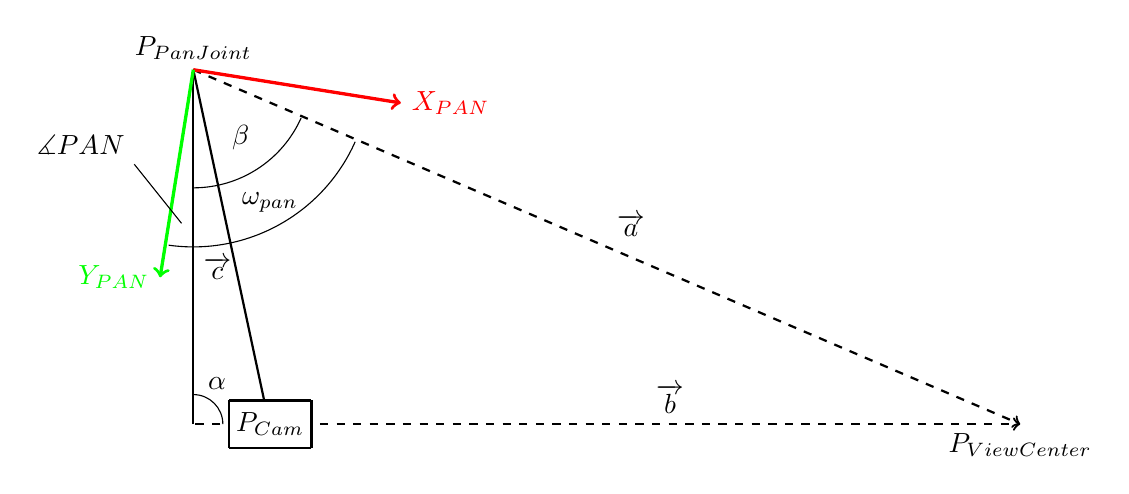
\begin{tikzpicture}[scale=1.5]
	\coordinate [label=above:${}P_{PanJoint}$](PAN) at (-1,3);
	\coordinate [label=center:${}P_{Cam}$](CAM) at (-0.35,0);
	\coordinate [](CAM_BASE) at (-1,0);
	\coordinate [label=below:${}P_{ViewCenter}$](VIEWCENTER) at (6,0);
	
	\draw [->,thick,dash pattern=on3pt off3pt] ([xshift=12pt]CAM) -- node[auto]{$\overrightarrow{b}$} (VIEWCENTER);
		\draw [-,thick,dash pattern=on3pt off3pt] ([xshift=-12pt]CAM) --(CAM_BASE);
	
	\draw [-,thick] (-0.7,0.2) -- (-0.7,-0.2);
	\draw [-,thick] (0,-0.2) -- (-0.7,-0.2);
	\draw [-,thick] (0,0.2) -- (-0.7,0.2);
	\draw [-,thick] (0,0.2) -- (0,-0.2);
	\draw [-,thick] (-0.4,0.2) -- (PAN);
	\draw [-,thick] (CAM_BASE) -- node[below right]{$\overrightarrow{c}$}(PAN);
	
	\draw [->,thick,dash pattern=on3pt off3pt] (PAN) -- node[auto]{$\overrightarrow{a}$} (VIEWCENTER) coordinate;
	
	\draw [->,very thick, red] (PAN) -- ([xshift=50pt,yshift=-8pt]PAN) node[right]{$X_{PAN}$};
	\draw [->,very thick, green] (PAN) -- ([xshift=-8pt,yshift=-50pt]PAN) node[left]{$Y_{PAN}$};
	
    	\draw (PAN)+(270:1) arc (270:336:1) ;
    \draw [color=black](PAN)+(305:0.7) node[rotate=0] {$\beta$};
    \draw (PAN)+(262:1.5) arc (262:336:1.5) ;
    \draw [color=black](PAN)+(300:1.3) node[rotate=0] {$\omega_{pan}$};
    
    	\draw (CAM_BASE)+(0:0.25) arc (0:90:0.25) ;
    \draw [color=black](CAM_BASE)+(60:0.4) node[rotate=0] {$\alpha$};
    \draw [-] (-1.1,1.7) -- (-1.5,2.2) node[above left]{$\measuredangle{}PAN$};
	
	\end{tikzpicture}
		\caption{Top perspective on the mild platforms pan-joint and the target view point. In the actual implementation, this plane will be called "viewTriangleXYPlane".} 
\end{figure}

In the above sketch, $\overrightarrow{c}$ represents the normal vector from the pan-joint to the plane, in which the camera position may move when rotating it around the tilt axis. This requires the assumption, that the tilt joint axis stands orthogonally to the Z axis. The length $\overrightarrow{c}$ is constant for all tilt angles and can therefore be precalculated.

As $\overrightarrow{c}$ stands orthogonal on the plane on which the camera moves, it can be assumed that $\alpha{}=90\degree$.

Side $\overrightarrow{a}$ represents the vector from pan joint to the actual view target point, which is then projected on the XY-plane.

Since we assume that $\overrightarrow{c}$ stands orthogonally on $\overrightarrow{b}$, $\norm{\overrightarrow{b}}$ can be determined as:

\begin{equation}
\norm{\overrightarrow{b}} = \sqrt{\norm{\overrightarrow{c}}^{2}-\norm{\overrightarrow{a}}^2}
\end{equation}

Once $\norm{\overrightarrow{b}}$ has been determined, the angle $\beta$ can be calculated using the law of cosines:

\begin{equation}
\begin{aligned}
\norm{\overrightarrow{b}}^2 = \norm{\overrightarrow{a}}^2 + \norm{\overrightarrow{c}}^2 - \norm{\overrightarrow{a}}*\norm{\overrightarrow{c}}*cos(\beta) \\
\implies 
\beta = acos(\frac{\norm{\overrightarrow{b}}^2 - \norm{\overrightarrow{a}}^2 - \norm{\overrightarrow{c}}^2}{\norm{\overrightarrow{a}}*\norm{\overrightarrow{c}}})
\end{aligned}
\end{equation}

To get the actual pan angle, the rotation of the pan joint relative to $\overrightarrow{b}$ in the 2D-projection $\omega$ has also to be taken into account.

It can be calculated by 

\begin{equation}
\omega_{pan}=\frac{\pi}{2}-asin(\frac{\langle\overrightarrow{a},\overrightarrow{y}_{pan}\rangle}{\norm{\overrightarrow{a}}*\norm{\overrightarrow{y}_{pan}}})
\end{equation}

where $\overrightarrow{y}_{pan}$ represent the Y-Axis of the pan joint's coordinate system.

Using these results, the actual pan angle $\measuredangle{}$Pan will be determined by:

\begin{equation}
 \measuredangle{}Pan=\omega_{pan}-\beta
\end{equation}


\section{Calculate $\measuredangle{}$Tilt}

Using the Pan-Angle from the previous step, the pose of the tilt joint in world coordinates can be easily calculated. Using this coordinate frame, another projection plane can used to determine the required tilt angle. This projection plane is orthogonal to the tilt joint's X-axis.

\begin{figure}[H]
	\centering\begin{tikzpicture}[scale=1.5]
		\coordinate [label=below:${}P_{TiltJoint}$](TILT) at (-1,-2);
		\coordinate [label=center:${}P_{Cam}$](CAM) at (-0.35,0);
		\coordinate [label=right:${}P_{ViewCenter}$](VIEWCENTER) at (6,0);


		\draw [-,thick] (-0.7,0.2) -- (-0.7,-0.2);
		\draw [-,thick] (0,-0.2) -- (-0.7,-0.2);
		\draw [-,thick] (0,0.2) -- (-0.7,0.2);
		\draw [-,thick] (0,0.2) -- (0,-0.2);
		\draw [-,thick] (-0.4,-0.2) -- node[above right]{$\overrightarrow{b}$}(TILT);
			
			
	\draw [->,thick,dash pattern=on3pt off3pt] (0,0) -- node[auto]{$\overrightarrow{c}$} (VIEWCENTER);
	
		\draw [->,thick,dash pattern=on3pt off3pt] (TILT) -- node[auto]{$\overrightarrow{a}$} (VIEWCENTER) coordinate;

		\draw [->,very thick, red] (TILT) -- ([xshift=30pt]TILT) node[right]{X} ;
		\draw [->,very thick, blue] (TILT) -- ([yshift=30pt]TILT) node[above]{Z};
		
		\draw (CAM)+(252:0.7) arc (252:360:0.7);
		\draw [color=black](CAM)+(300:0.5) node[rotate=0] {$\alpha$};
    		
    		\draw (TILT)+(16:0.7) arc (16:72:0.7);
		\draw [color=black](TILT)+(45:0.5) node[rotate=0] {$\gamma$};
		
	\end{tikzpicture}
		\caption{Side perspective on the mild platforms tilt-joint and the target view point} 
\end{figure}

In this case, $\overrightarrow{a}$ is simply the distance between the tilt joint and the target view center point. Furthermore, $\overrightarrow{b}$ as well as the angle $\alpha$ can be precalculated using the robots kinematic chain.

Using this, the projected distance between the camera and the target view center $\norm{\overrightarrow{c}}$ can be determined using the law of cosines:

\begin{equation}
\begin{aligned}
\norm{\overrightarrow{a}}^2 = \norm{\overrightarrow{b}}^2 + \norm{\overrightarrow{c}}^2 - \norm{\overrightarrow{b}}*\norm{\overrightarrow{c}}*cos(\beta) 
\implies \\
\norm{\overrightarrow{c}} = -\frac{\norm{\overrightarrow{b}}*cos(\alpha)}{2} \pm \sqrt{(\frac{\norm{\overrightarrow{b}}*cos(\alpha)}{2})^2-(\norm{\overrightarrow{a}})^2+(\norm{\overrightarrow{b}})^2}
\end{aligned}
\end{equation}

In the above equation, the positive case can always be assumed to be the correct solution (the negative case would represent the camera facing the target with its backside), so we can now use $\norm{\overrightarrow{c}}$ to determine the $\gamma$ using the law of cosines like before:

\begin{equation}
\gamma = acos(\frac{\norm{\overrightarrow{c}}^2 - \norm{\overrightarrow{a}}^2 - \norm{\overrightarrow{b}}^2}{\norm{\overrightarrow{a}}*\norm{\overrightarrow{b}}})
\end{equation}

By simply substracting an angle offset $\delta_{tilt}$, the actual tilt angle required to focus the target view point is acquired:

\begin{equation}
\measuredangle{}Tilt = \gamma-\delta_{tilt}
\end{equation}
\printbibliography


\end{document}